\chapter{Numerical Methods and Simulation}

\newpage

\section{Matlab}
\url{https://www.egr.msu.edu/aesc210/systems/MatlabCheatSheet.pdf} \newline
\textbf{Viktiga syntax/comandons}
\begin{verbatim}
  zeros(1,N);  % creates a vector of N lenght
  zeros(N); % creates a matrix of N*N size
  mean([1 2 2 3]); % avrage value with is 2 in this cases
  vector(line,row); 
  hold on % holes the current plot and plots new over old
  xlable("some x lable") % naming the plot x axis
  ylable("some y lable") % naming the plot y axis
  title("some title for the plot")
  ode45(@(t,y) 2*t, tspan, y0);
  [t,y] = ode15s(@(t,y) myode(t,y,A,B), tspan, y0);
  linespace(StartPoint, EndPoint); % gemerates a row of vector
  fzero(func, currentValueOfFunction, optimeset('Tolx', 1e-02)); 
  [0; 1; 2]; % Vector not array
  numel(x0); % the number of dimension of vector
  repmat(x0(i), N, 1); % generate values 
  cumsum(rand) % the cumulative sum of Noise starting at the beginning of the first array dimension in Noise whose size does not equal 1.
\end{verbatim}


\section{Aritmatic}
När beräkningar sker så andvänder den inte exaxta värdet utan konverterar till binärt och där med får
ungefär väde. Räknar inte med bråk utan floting point.

(Mantissa $m$ hur många index det finns för $d_i$), (Bas $\beta$), (exponent $e$). Man kan skriva ett decimaltal så här: $x=m\beta^e$.
(Normaliserad form) är då första talet är en siffra ($1.23*10^{-1}$ ej $0.123$)
$m=d_0*2^0+d_1*2^{-1}+d_2*2^{-2}+ \ldots +d_n*2^{-p}$. Normaliserad form ger att $d_0$ i altid 1 i binär form och
därmed så behöver man inte sparra den. Den kallas hidden bit.

$E$ andvänds för att konvertera till en normal form tex $0.d_1d_2..d_{52}\cdot{2^{-1022}}$ i subnormal form blir
$1.d_1d_2..d_{52}\cdot{2^{E-1022}}$, där $E=1$, i normal form.

\subsection{IEEE}
IEEE, ger en standard till olika representationer.
\begin{itemize}
  \item Singleprecision (32 bit, enkel precision)
  \item Double precision (64 bit, dubbel precision)
  \item Extendedprecision (80 bit, utökad precision)
\end{itemize}
matlab andvänder double presission.
Tal som är störe än realmax i matlab blir Inf och tal som är ogiltiga är NaN.

\subsection{Maskinepsilon}
Def: Gapet mellan $1$ och nästa representerbara tal, minsta talet $\epsilon_M$ för vilket
gäller $1+\epsilon_M > 1$. Det är ett mått på tals systemetsprecision. $\epsilon_M \approx 10^{-16}$

\begin{lstlisting}[language=Python]
  if(x == y)
  ifabs((x-y)/x)<tol
\end{lstlisting}

\subsection{Diskretiseringsfel}
Vid exempelet när man beräknar derivatan så är \textit{avrundningsfelet} den dominanta. Medans
vid Störe h så dominerar \textit{Diskretiseringsfel}

\section{ODE}
Skillnaden mellan metod och modell är att moted är hur man gör, 
medans modell är strukturen av företelsen.
För att man ska kunna lösa en ode så behöver den vara en entydlig 
lösning samt små skilnader på inparametrar ger littet skilnad i resultat.

\textbf{Löser med ode45}
\begin{verbatim}
  %%%%%%%%% myODE.m
  function yprim = myODE(t,y)
    % y'(t) = 3y(t)(1-y(t))
    yprim = 3*y*(1-y)
  end
  %%%%%%%%% script.m
  % Tidsintervall mellan 0 till 10
  % Begynnelse vilkor på 0.1
  [t,y] = ode45(@myODE, [0 10], 0.1)
  plot(t,y)
\end{verbatim}

\subsection{Numeriska metoder}
När numrerisk fel är mindre än propotionelit ex $h^2$ då blir avrundningsfelet den dominanta

\textbf{Implecita metoder}
Ovilkoliga stabilita.

\textbf{Explicit metoder}
Kan vara effectivara, fämst för icke styva ode'r
 
\subsubsection{Euler framåt (explicit metod)}
Tar lutningen vid punkten man är i och beräknar värdet för ett givet steg.

\textbf{Ex:}
\begin{align*}
  &\quad  \frac{y'(x)}{x} - y\sin{(x)} = 0, \; y(0)=1 \\
  &\quad  \text{Euler framåt: } y_{k+1} = y_k h_kf(t_k,y_k) \\
  &\quad  \\
  &\quad  y'(x) = xy\sin{(x)}, \; f(x,y) = xy\sin{(x)} \\
  &\quad  y_{i+1} = y_i + hf(x_i,y_i) = y_i+hx_i\cdot{y_i\sin{(x_i)}} \\
  &\quad  \text{Väljer $h=0.1$ (h är steget mellan det approximerade linjerna)} \\
  &\quad  y_0 = 1 \\
  &\quad  y_1 = y_0+hx_0y_0\sin{(x_0)} = 1+0.1\cdot0\cdot1\sin{0} = 1 \\
  &\quad  y_2 = y_1+hx_1y_1\sin{(x_1)} = 1+0.1\cdot0.1\cdot1\sin{0.1} = 1.001 \\
  &\quad  y_3 = y_2+hx_2y_2\sin{(x_2)} = 1.001+0.1\cdot0.2\cdot1.001\sin{0.2} = 1.005 \\
  &\quad  * \\
  &\quad  y_{10} = 1.2895 \\
  &\quad  \\
  &\quad  \text{Aritmetiska lösnig (Räknat ut exakta värdet) }
  y(1)=e^{\sin{(1)-1-\cos{(1)}}} = 1.3514 \\
  &\quad  \text{Fel} = 1.2895-1.3514 = -0.0619 \\
  &\quad  \text{Väljer } h=0.01, \; y_{100} = 1.3448 \text{ Fel} = -0.00669 \\
  &\quad  \text{Väljer } h=0.01, \; y_{1000} = 1.35076 \text{ Fel} = -6.74\cdot10^{-4} \\
  &\quad  \text{Vi ser att felet är propotionelit mot steg ($h$). Fel } \alpha \; h \\
\end{align*}

\subsubsection{Euler bakåt (implicit metod)}
Tar lutningen ett steg framåt.

\textbf{Ex:}
\begin{align*}
  &\quad  \text{Euler bakåt: } y_{k+1} = y_k h_kf(t_{k+1},y_{k+1}) \\
  &\quad  \\
  &\quad  y'(x) = xy\sin{(x)}, \; y(0)=1 \\
  &\quad  y_{i+1} = y_i + hx_{i+1}y_{i+1}\sin{(x_{i+1})} \\
  &\quad  \Rightarrow y_{i+1} -hx_{i+1}\cdot{y_{i+1}}\sin{(x_{i+1})} = y_i \\
  &\quad  \Rightarrow y_{i+1} = \frac{y_i}{1 -hx_{i+1}\sin{(x_{i+1})}} \\
  &\quad  \text{Väljer $h=0.1$} \\
  &\quad  y_0 = 1 \\
  &\quad  y_1 = \frac{y_0}{1 -hx_{1}\sin{(x_{1})}} = \frac{1}{1 -0.1\cdot0.1\cdot\sin{0.1}}
        = 1.000999 \\
  &\quad  y_2 = \frac{y_1}{1 -hx_{1}\sin{(x_{1})}} = 1.00499 \\
  &\quad  * \\
  &\quad  y_{10} = 1.42556 \\
  &\quad  \\
  &\quad  \text{Aritmetiska lösnig: } y(1)=e^{\sin{(1)-1-\cos{(1)}}} = 1.3514 \\
  &\quad  \text{Fel} = 1.42556-1.3514 = +0.07412 \\
  &\quad  \text{Väljer } h=0.01, \; y_{100} = 1.35825 \text{ Fel} = +0.00681 \\
  &\quad  \text{Väljer } h=0.001, \; y_{1000} = 1.35211 \text{ Fel} = +6.75\cdot10^{-4} \\
  &\quad  \text{Vi ser att felet är propotionelit mot steg ($h$). Fel } \alpha \; h \\
\end{align*}

\subsubsection{Trapetsmetoden (implicit metod)}
Trapetsmetoden uses the avrage value of the euler framåt and backåt.

\textbf{Ex:}
\begin{align*}
  &\quad  \text{Trapetsmetoden } y_{i+1}=y_i + 0.5h_i(f(t_i,y_i) + f(t_{i+1},y_{i+1}))
  &\quad  y'=xy\sin(x) \\
  &\quad  y_{i+1} = y_i+h/2(x_i\cdot{y_i}\sin(x_i)+x_{i+1}y_{i+1}\sin{(x_{i+1})}) \\
  &\quad  \Rightarrow y_{i+1} = \frac{y_i+h/2(x_i\cdot{y_i}\sin(x_i))}{1-h/2(x_i)+\sin{x_{i+1}}}
  &\quad  y_0=1 \; h=0.1 \\
  &\quad  y_1=0.00499 \\
  &\quad  * \\
  &\quad  y_{10}=1.3343, \text{ Fel} = 0.00286 \\
  &\quad  \text{Väljer } h=0.01, \; y_{100} = 1.35147 \text{ Fel} = +2.86\cdot10^{-5} \\
  &\quad  \text{Väljer } h=0.001, \; y_{1000} = 1.3514275 \text{ Fel} = +2.86\cdot10^{-7} \\
  &\quad  \text{Vi ser att felet är propotionelit mot steg ($h$). Fel } \alpha \; h^2 \\
\end{align*}

\subsubsection{Heuns metod (explicit metod)}
Trapetsmetoden ger bra approximationer men är dock implicit vilket gör det svårt för icke linjära
ODE. Det kan huens metod lösa genom att approximera implicita delen.

\textbf{Metod:}
\begin{align*}
  &\quad  \text{Huens metod } y_{i+1} = y_n + h_n/2[f(t_n,y_n) + f(t_{n+1},hf(t_n,y_n))] \\
  &\quad  \\
  &\quad  k_1=f(x_i,y_i) \\
  &\quad  k_2=f(x_i,y_i) \\
  &\quad  y_{i+1} = y_i+h(k_1+k_2) \\
  &\quad  \text{Vi ser att felet är propotionelit mot steg ($h$). Fel } \alpha \; h^2 \\
\end{align*}

\textbf{Ex:}
\begin{align*}
    &\quad  y'=10\cdot{y}(1-\frac{y}{1000}), \; y(0)=1, \; h=0.1 \\
    &\quad  \\
    &\quad  \text{i. löser ut } y'(t) \\
    &\quad  y'(t) = 10\cdot{y}(1-y/1000) \\
    &\quad  \\
    &\quad  \text{ii. Heuns metod, utryck för } y_{i+1} \\
    &\quad  y_{n+1} = y_n+h_n/2(k_1+k_2) \\
    &\quad  \\
    &\quad  \text{iii. Beräknar } \\
    &\quad  k_1 = f(t_0,y_0) = 10\cdot{1}(1-\frac{1}{1000}) = 9.99 \\
    &\quad  k_2 = f(t_1,y_0+hk_1) = f(t_1,1.999)= 10\cdot{1.999}(1-\frac{1.999}{1000}) = 19.99(0.998001) \approx 19.95 \\
    &\quad  \Rightarrow y_1 = y_0 + h_0/2(k_1+k_2) = 1+0.05(k_1+k_2) \approx 2.497 \\
\end{align*}


\subsubsection{Runge-Kutta (explicit metod)}
Runge-Kutta är noggran numrerisk approximering, betydligt bättre än 
euler framåt/backåt. Man berärknar 4 lutningar och tar typ medelvärdet av dem.
\begin{figure}[h]
    \vspace{10mm}
    \centering
    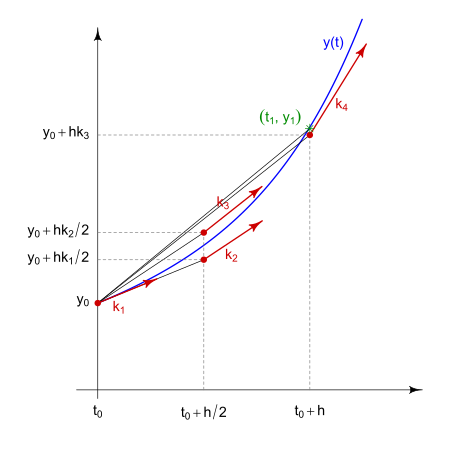
\includegraphics[width=8cm, height=6cm]{image/Runge-Kutta_slopes.png}
    \caption{Runge-Kutta}
\end{figure}

\textbf{Ex:}
\begin{align*}
    &\quad  y'(t)-y(t)-t=0, \; y(0)=0, \; h=0.1, \; \text{RK 1-steg} \\
    &\quad  \\
    &\quad  \text{i. löser ut } y'(t) \\
    &\quad  y'(t)=y(t)+t \Rightarrow f(t,y) = y+t \\
    &\quad  \\
    &\quad  \text{ii. Runge-Kuttas, utryck för } y_{i+1} \\
    &\quad  y_{n+1} = y_n+\frac{1}{6}h(k_1+2k_2+2k_3+k_4) \\
    &\quad  \\
    &\quad  \text{iii. Beräknar } \\
    &\quad  k_1 = f(t_0,y_0) = y_0 + t_0 = 0 \\
    &\quad  k_2 = f(t_0+h/2,y_0+hk_1/2) = f(0.05,0) = 0.05 \\
    &\quad  k_3 = f(t_0+h/2,y_0+hk_2/2) = f(0.05,0.0025) = 0.0525 \\
    &\quad  k_4 = f(t_0+h,y_0+hk_3) = f(0.1,0.00525) = 0.10525 \\
    &\quad  k = (k_1+2k_2+2k_3+k_4)/6 = (0+2*0.05+2*0.0525+0.10525)/6=0.31025/6 \\
    &\quad  y_1 = y_0 + h\cdot(0.31025/6) = 0.1\cdot(0.31025/6) \approx 0.00517 \\
\end{align*}

\newpage
\subsection{Högre årdningens ODE}
\begin{align*}
  &\quad  x''(t) = -\frac{x(t)}{(\sqrt{x(t)^2+y(t)^2})^3} \\
  &\quad  y''(t) = -\frac{y(t)}{(\sqrt{x(t)^2+y(t)^2})^3} \\
  &\quad  \\
  &\quad  \\
  &\quad  \text{Låt } \overline{u} =  \begin{pmatrix} u_1 \\ u_2 \\ u_3 \\ u_4 \end{pmatrix} \\
  &\quad  u_1 = x,  \; u_1' = u_2 \\
  &\quad  u_2 = x', \; u_2' = -\frac{u_1}{(\sqrt{u_1^2+u_2^2})^3} \\
  &\quad  u_3 = y,  \; u_3' = u_4 \\
  &\quad  u_4 = y', \; u_4' = -\frac{u_3}{(\sqrt{u_1^2+u_2^2})^3} \\
  &\quad  \overline{u}' =
  \begin{pmatrix}
      u_2 \\
      -\frac{u_1}{(\sqrt{u_1^2+u_2^2})^3} \\
      u_4 \\
      -\frac{u_3}{(\sqrt{u_1^2+u_2^2})^3} \\
  \end{pmatrix} \\
\end{align*}

Löser i matlab:\newline
Ställer upp ODE i separat fil
\begin{lstlisting}
    function u_out = satellitODE(t,u)

    u_out = [ u(2);
              -( u(1)/( sqrt( u(1)^2 + u(2)^2 )^3 ) );
              u(4);
              -( u(3)/( sqrt( u(1)^2 + u(2)^2 )^3 ) )];
\end{lstlisting}

Sedan kan man kalla med följande script
\begin{lstlisting}
    tidsintervall = [0, 100];
    
    % satelitens position (x(0),y(0))
    % satelitens hastighet (x'(0), y'(0))
    u0 = [0; 22223; 17000; 100];

    [t, u] = ode45(@satellitODE, tidsintervall, u0, odeset)

    plot(t,u)
\end{lstlisting}



\newpage
\section{Analys}
\textit{Styv} mångra ädringar under kort tid.
\textit{Adaptivt steglängdsval} som ode15s och ode45. Anpassar steglängd efter styvhet.

\subsection{Analys av metoder}
\begin{align*}
  &\quad  \text{ODE: } y'=f(t,y) \\
  &\quad  \text{Metod: } y_{i+1} = y_i +h\cdot{\Psi_k}(t_i, y_{i+1}, y_1) \\
\end{align*}

\subsection{Konsistent}
Metoden är konsistent med ode'n om:
\begin{align*}
  &\quad \lim_{h\to0} \Psi_h = \Psi_0(t_i,y_i) = f(t_i,y_i) \\
\end{align*}

\subsection{Rättstält}
\begin{align*}
  || \overline{F}(x,\overline{u})-\overline{F}(x,\overline{z}) \leq L\cdot||\overline{u}-\overline{z}|| \\
  L = max||J(x,\overline{u})|| \;\;\; \text{ -jacobianen}
\end{align*}

\subsection{Noggrannhetsordning}
Låt $\phi(0)$ vara en funkion som uppfyller ode'n och är tillräklight deriverbar.
Bilda lokala trunkteringsfelet
\begin{align*}
  &\quad \tau = \phi(t_{i+1})-(\phi(t_i)+h\Psi_h(\phi(t_{i+1}),\phi(t_i))) \\
\end{align*}
och taylorutveckla kring $t_i$ och låt $h\to0$. 
Om $\Psi\to{C\cdot{h^{P+1}}}$ (dominerande term)
Så har metoden noggranhetsordning P
\begin{align*}
  &\quad \tau_h\to{C\cdot{h^{P+1}}} \Leftrightarrow \frac{\phi(t_{i+1})-\phi(t_i)}{h}+\Psi_h(t_i,\phi(t_{i+1}),\phi(t_i))\to{Ch^P} \\
\end{align*}


\textbf{Exemple: Visa nu att Euler bakåt (implicit Euler) har noggranhetsordning 1} \newline
Lokala trunkteringsfelet $\tau$ för implicit Euler metod är:
\begin{align*}
  \tau = y(t_{k+1})-y(t_k)-hf(t_{k+1},y(t_{k+1}))
\end{align*}

Vi kan då ersätta $f(t_{k+1},y(t_{k+1}))$ med $y'(t_{k+1})$ (ode'n) vilket ger:
\begin{align*}
  \tau = y(t_{k+1})-y(t_k)-hy'(t_{k+1})||
\end{align*}

Sedan analyserar vi det lokala trunkteringsfelet genom taylorutveckla
den implecita delen av utryck vid punkt $t=t_k$.
Där av så är $t_{k+1}=t_k+h$
\begin{align*}
  \tau &= y(t_{k+1})-y(t_k)-hy'(t_{k+1})  \\
  &= y(t_k)+hy'(t_k)+\frac{h^2}{2}y''(t_k)+O(h^3) \\
  &-y(t_k)-h(y'(t_k)+y''(t_k)+O(h^2)) \\
  &= \big( \frac{h^2}{2} - h^2 \big)y''(t_k)+O(h^3) = O(h^2)
\end{align*}
Därmed så är det lockala trunkteringsfelet $O(h^2)$ och nogranhets ordningen
$p$ i $\tau_{h}=Ch^{p+1}\Rightarrow p=1$. V:S:V 

\newpage

\subsection{Stabilitet}
Vi undersöker Stabilitet på testekvationen
\begin{align*}
  &\quad  y'=\lambda y \;\;\; \text{ där } re(\lambda)\leq 0 \\
\end{align*}

\textbf{Euler framåt} har stabilitetsområdet
\begin{align*}
  &\quad  |1+h\lambda|\leq1 \\
\end{align*}
Reella $\lambda$ ger $-1\leq1+\lambda h \Leftrightarrow h\leq\frac{-2}{\lambda}$

\textbf{Euler bakåt} har stabilitetsområdet
\begin{align*}
  &\quad  \frac{1}{|1-\lambda h|} \leq 1 \text{  dvs ovilkorligt stabil} \\
\end{align*}

\textbf{Exemple: Visa nu att Euler bakåt (implicit Euler) är ovillkorligt stabil} \newline

Testekvationen ses som sådan:
\begin{align*}
     y' &= \lambda\cdot y\\
%   y(t) &= e^{\lambda\cdot t} \\
y_{i+1} &= y_i + hf(t_{i+1}, y_{i+1}) \\
\end{align*}

Euler bakåt:
\begin{align*}
y_{i+1} &= y_i + h\cdot f(t_{i+1}, y_{i+1}) \\
	&= y_i + h\lambda \cdot y_{i+1}
\end{align*}

Vi bryter ut $y_{i+1}$:

\begin{align*}
y_{i+1} - h\lambda \cdot y_{i+1} &= y_i \\
y_{i+1} \cdot (1 - h\lambda) &= y_i \\
y_{i+1} &= \frac{1}{1 - h\lambda} \cdot y_i
\end{align*}

Då ser vi att vårt stabilitetsvillkor är följande:

\begin{align*}
\left| \dfrac{1}{1-h\lambda} \right| \le 1
\end{align*}

Vi antar (enligt uppgift) att $\lambda$ är reellt och att $Re(\lambda) \le 0$. Detta medför att följande alltid kommer vara mindre än 1. Nämnaren blir större än täljaren för alla värden på $\lambda$.
\begin{align*}
1 - h\lambda \ge 1 \Rightarrow \left| \dfrac{1}{1-h\lambda} \right| \le 1
\end{align*}

för alla våra värden på $\lambda$. På grund av detta vet vi att oavsett värde på $h$ så kommer den numeriska lösningen vara stabil, d.v.s ovillkorligt stabil.


\newpage
\subsection{Stabilitet generella ekvationer}
Betrakta små rörelser av $y$ (momentant)
\begin{align*}
  &\quad  y=\tilde{y}+z \;\;\; \text{  z-litet, $\tilde{y}-konstant$} \\
  &\quad  z'=f(t,\tilde{y}) \approx f(t,\tilde{y})+z\cdot\dfrac{\delta f}{\delta y}(t,\tilde{y}) = C_1+C_2z
\end{align*}

\underline{Sats} om den numeriska metoden är stabil för alla 
\begin{align*}
  &\quad  C_2=\dfrac{\delta f}{\delta y}(t,\tilde{y}) \\
\end{align*}
i lösningsområdet på testekvationen $(\lambda=C_2)$

\subsection{Stabilitet för system}
\begin{align*}
  &\quad  \overline{u} = F(t,\overline{u}) \; \overline{u} \; F(t,\overline{u})
  \begin{bmatrix}
    f_1(t,\overline{u})\\
    f_2(t,\overline{u})\\
    .\\
    f_3(t,\overline{u})\\
  \end{bmatrix}\\
  &\quad  \text{Betrakta små rörelser (mementant)} \\
  &\quad  \text{låt } \overline{u}=\tilde{u}+\overline{z} \approx F(t,\tilde{u})+F'(t,\tilde{u})\overline{z} \\
  &\quad  \text{där } F'(t,\tilde{u})=
  \begin{bmatrix}
    \dfrac{\delta f_1}{\delta u_1} & \dfrac{\delta f_1}{\delta u_2} & ... & \dfrac{\delta f_1}{\delta u_n} \\
    \dfrac{\delta f_1}{\delta u_1} & \dfrac{\delta f_1}{\delta u_2} & ... & \dfrac{\delta f_1}{\delta u_n} \\
    . & & & \\
    \dfrac{\delta f_n}{\delta u_1} & \dfrac{\delta f_n}{\delta u_2} & ... & \dfrac{\delta f_n}{\delta u_n} \\
  \end{bmatrix}\\
  &\quad F(t,\tilde{u}) \text{ -konstantlägre odningens term påverar ej stabiliteten}\\
\end{align*}

Studera: $\overline{z}'=A\overline{z}$ där $A=F'(t,\tilde{u})$ (konstant matris)
Låt $\overline{w}=s^{-1}\overline{z}$ $\Leftrightarrow$ $\overline{z}=S\overline{w}$
$\Rightarrow S\overline{w}'= AS\overline{w}$ $\Leftrightarrow$ $\overline{w}'=S^{-1}AS\overline{w}$
där $D=S^{-1}AS$. Vi väljer $S$ så att $D$ blir diagonal med $A$'s egenvärde i diagonalen,
$\overline{w}'=Dw$
\begin{align*}
\Rightarrow 
\begin{cases}
  w_1'=\lambda_1w_1\\
  w_2'=\lambda_2w_2\\
  .\\
  w_n'=\lambda_nw_n\\
\end{cases}\,.
\end{align*}

\underline{sats}: Om den numeriska metoden är stabil för $w_i'=\lambda_iw_i$, alla $\lambda_i=\lambda(t,\tilde{u})$
i lösningsområdet så ör deb stabil för $\overline{u}'=F(t,\overline{u})$
$\Rightarrow$ Utanför stabilitetsanalysen på testekvation $y'=\lambda y$ men med $\lambda_i(t,\tilde{u})$
(egenvärdena till jacobianen)

\underline{Not}: $\lambda$ - kan vara komplext (äen om $\overline{u}$ och $F(t,\overline{u})$ är reela)

% What dose region of stability mean (för vilka värden är metoden stabil Im och Re-del)
% stabilitet för bunge jump. Ha med annalys exemplel om det inte finns. Blir svårare med komplexa rötter.
% explodera
% aplikations faktorn
% man kan numeriskt annylisera stabiliteten hos RK

\newpage
\section{Stokastiska metoden}
\begin{itemize}
  \item Deterministisk metoder: Det vi tidigare kållat på. Får samma svar för sama input
  \item Stokastiska metoder: Varierar för same input, då slumpen spellar roll.
\end{itemize}

\subsection{Monte Carlo}
\begin{verbatim}
  Indata: N (antal försök)
  for i=1:N
    Gör en stokastisk simulering
    resultat(i)=resultat av simulering ovan
  end 
  slutresultat = mean(resultat)
\end{verbatim}

\textit{Ensemble-prognoser} är att man kör flertal gånger och kan ta medelvärdet
för att få den troliga lösningen men sen också gemföra med och se hur stora fel/
osäkerhet är prognosen. \newline

\textit{Initialtilståndet} \newline

\underline{Matlab} har flera olika slumptals genererare
\begin{itemize}
  \item \"rand\": slumptal mellan 0 och 1
  \item \"randn\": normalfördelade slumptal
\end{itemize}

\underline{Nogrannhetsordning} Monte Carlo är oberonde av dimensioner 
(vilket ex trapetsmetoden inte är).
\begin{align*}
  \text{Trapetsmetoden - Fel } &\sim O(n^{-2/d})  \\
  \text{MC - Fel } &\sim O(1/\sqrt{N}) 
\end{align*}


\newpage

\subsection{Invers Transform Sampling (ITS)}
ITS är en algorithm för att generera slumptal ut ifrån 
en given fördelning.

Cumulative distribution function (CDF): is that you take the 
primitive function of a distribution. 
Man kan då bestäma $\tau$ som är tiden för reaktion ska ske.

\textbf{Exempel: ITS}
\begin{align*}
  &f_{\lambda}(x)=\frac{1}{\lambda}e^{-x/\lambda} \\
  &\\
  \text{1. Hitta primitiva funktionen }&   \\
  & F_{\lambda(x)} = {\int^x}_0 \frac{1}{\lambda}e^{-t/\lambda}dt 
  = {[-e^{-t/\lambda}]^x}_0
  = 1-e^{-x/\lambda} \\
  \text{2. Hitta inversen }& \\
  & F^{-1}: \text{Löser } y=1-e^{-x/\lambda} \\
  & y-1 = -e^{-x/\lambda} \Rightarrow ln(1-y)=-x/\lambda \Rightarrow x=-\lambda ln(1-y) \\
  &\text{Vilket är exponentialfördelad}
\end{align*}

\subsubsection{Diskret slumptalsfördelning}

\textbf{Exempel: ITS Diskret slumptalsfördelning}
\begin{align*}
  \text{1: Röd; } P_1 &= 0.45 \\
  \text{2: Gul; } P_2 &= 0.10 \\
  \text{3: Grön; } P_3 &= 0.45 \\
  u&=0.61 \\
  \\
  &\text{ITS innebär i den diskreta versionen att $r$,} \\
  &\text{numret på nästa utfall, ska väljas som det minsta tal $x$} \\
  &\text{så att } F(x)\leq u \text{, där $F(x)$ är den kumulativa fördelningsfunktionen.} \\
  &\text{Med de givna värdena kan $F(x)$ representeras av vektorn} \\
  \\
  F &= 
  \begin{bmatrix}
    0.45 \\
    0.45 + 0.10 \\
    0.45 + 0.10 + 0.45 
  \end{bmatrix} =
  \begin{bmatrix}
    0.45 \\
    0.55 \\
    1.00 
  \end{bmatrix} \\
  &\text{Vi ser att $F(3)$ är den första som är störe än $0.61$.} \\
  &\text{Slutsatsen är att det kommer då vara $r=3$, färgen grön som slumpas fram.}
\end{align*}


\newpage

\subsection{Gillespie algorithm/Stochastic Simulation Algorithm (SSA)}
Simulering av reaktioner oftast i kemiska kontext.

\textbf{Exemple}
\begin{align*}
    S'(t) &= -\beta\frac{I(t)}{N}S(t) \\
    I'(t) &= \beta\frac{I(t)}{N}S(t) -\gamma I(t) \\
    R'(t) &= \gamma I(t) \\
\end{align*}

\textit{Reaktioner}:
\begin{center}
\begin{tabular}{ c c }
 $r_1$: & $\beta\dfrac{I(t)}{N}S(t)$  \\  
 $r_2$: & $\gamma I(t)$  \\    
\end{tabular}
\end{center}

\textit{Reaktionsmatris}:
\begin{center}
\begin{equation*}
\begin{array}{c c} &
\begin{array}{c c c} S(t) & I(t) & R(t) \\
\end{array}
\\
\begin{array}{c c}
r_1 \\
r_2 
\end{array}
&
\left[
\begin{array}{c c c}
\; -1 \; & \;  1 \; & \; 0 \; \\
\;  0 \; & \; -1 \; & \; 1 \; 
\end{array}
\right]
\end{array} = R
\end{equation*}
\end{center}

Då har vi även reaktionshastighets-vektorn som följande. \newline
Samt att $C = \{ \beta, \gamma, N \}$.

\begin{equation*}
    \mathbf{P(\Vec{y}, C)}=
    \begin{bmatrix}
        C(1)\dfrac{y(1)}{C(3)}y(2) \\
        C(2)y(1)
    \end{bmatrix}
\end{equation*}

I matlab: 

\section{Ordlista}
\begin{itemize}
  \item \textit{Adaptiv steglängd}: Att den numeriska metoden i varje steg automatiskt ställer in
steglängden så att det uppskattade felet blir lägre än toleransen.
  \item \textit{Cumulative distrubution function}: du finner primitiva functionen av distributionen.
  \item \textit{Deterministisk metoder}: En algoritm utan slumpmoment, så att utdata beror entydigt på
indata.
  \item \textit{Deterministisk modell}: En modell utan slumpmoment, så att utdata beror entydigt på
indata.
  \item \textit{Diskretiseringsfel}: Vid exempelet när man beräknar derivatan så är
dominerar Diskretiseringsfel
  \item \textit{Explicit metod}: En metod för numerisk lösning av ODE, där högerledet i metoden
bara beror på kända värden.
  \item \textit{Global trunkteringsfelet}: Det sammanlagda felet i från det tidigare stegen med den numeriska metoden utgående från exakta
lösningen i senaste tidpunkten.
  \item \textit{Implecit metod}: En numerisk metod för lösning av ODE, där högerledet i metoden
innehåller $y_{i+1}$ , så att man måste lösa en ickelineär ekvation i varje
steg.
  \item \textit{ITS}: en algorithm för att generera slumptal ut ifrån en given fördelning
  \item \textit{Konsistent}: Den numeriska metoden går mot differentialekvationen då h går
mot noll.
 \item \textit{Kancellation}: Förlust av signifikanta siffror vid subtraktion mellan jämnstora
flyttal.
  \item \textit{Konvergens}: Den numeriska lösningen går mot den exakta lösningen då stegläng-
den h går mot noll.
  \item \textit{lockala trunkteringsfelet}: Felet i ett steg med den numeriska metoden utgående från exakta
lösningen i senaste tidpunkten.
  \item \textit{Mantissa}: bråkdelen i floting point
  \item \textit{Maskinepsilon}: Det relativa fel man får då tal lagras i en dator (eller när beräkningar utförs) beror på hur talen lagras internt i datorn.
  \item \textit{Monte Carlo-metod}: Upprepad stokastisk simulering samt statistik på de samlade re-
sultaten.
  \item \textit{Normalisering}: Konventionen att i flyttalsrepresentation ha precis en nollskild
siffra före "decimalpunkten" (så att flyttalsrepresentationen blir
entydig).
  \item \textit{Noggrannhetsordning}: h-potensen i globala trunkeringsfelet hos en numerisk metod för
lösning av ODE (där h är steglängden).
  \item \textit{Overflow}: Motsatsen till underflow.
  \item \textit{Stokastiska modell}: En modell med slumpmoment, så att utdata inte beror entydigt
på indata.
 \item \textit{Styv}: En ODE för vilken en explicit differensmetod behöver ta mycket
kortare steg för stabilitet än vad som skulle krävas för tillräcklig
noggrannhet.
  \item \textit{Stabilitet}: Störningskänsligheten hos den numeriska metoden.
  \item \textit{SSA/Gillespie algorithm}:
  \item \textit{Underflow}: Det som uppstår när vi försöker representera ett tal vars abso-
lutbelopp är mindre än det till beloppet minsta normaliserade
flyttalet.
  \item \textit{jacobianen}
\end{itemize}
